\chapter{Teoria de Hückel e sistemas conjugados}\label{ch:b2:huckel}

Ao hidrogenar o ciclo-hexeno, liberam-se \qty{119}{kJ} por mol. O benzeno, com
três ligações duplas em um anel de seis carbonos, deveria liberar três vezes
mais a caminho do ciclo-hexano; ele libera \qty{150}{kJ} a menos. Essa energia
que falta é a estabilidade de um anel \omterm{def:b2:huckel:aromatic}{aromático}, a razão pela qual o benzeno
resiste às adições que os alcenos sofrem. Em 1931, Erich Hückel a calculou com
um determinante, depois de reduzir a molécula a seus elétrons $\pi$ e a seus
vizinhos. Seu método é grosseiro, mas explica por que os anéis de seis
elétrons $\pi$ são especiais, por que as longas cadeias conjugadas absorvem luz
visível e onde uma molécula conjugada carrega suas cargas.

\begin{recall}
\Cref{ch:b2:diatomic-mos}: \omterm{def:b2:diatomic-mos:integrals}{integral de Coulomb} $\alpha$, \omterm{def:b2:diatomic-mos:integrals}{integral de ressonância}
$\beta$, \omterm{def:b2:diatomic-mos:integrals}{determinante secular}. \Cref{ch:b2:fragment-orbitals}: orbitais $\pi$ do
eteno e do alila. O volume do 1.º ano: sistemas conjugados, ressonância,
cromóforos e máximos de absorção.
\end{recall}

\section{O método de Hückel}

Em uma molécula conjugada plana, os orbitais $\sigma$ são simétricos e os
orbitais p perpendiculares ao plano, antissimétricos em relação a esse plano:
eles não se misturam (\cref{prop:b2:diatomic-mos:symmetry}), e os elétrons $\pi$
podem ser tratados isoladamente.

\begin{definition}[Método de Hückel]\label{def:b2:huckel:method}
O \emph{método de Hückel}\index{metodo de Huckel@método de Hückel} calcula os orbitais $\pi$ de um
sistema conjugado plano como combinações $\psi = \sum_r c_r p_r$ de um orbital p
por átomo, com as aproximações: sobreposições $S_{rs} = 0$ para $r \neq s$ (e 1 para $r =
s$); \omterm{def:b2:diatomic-mos:integrals}{integrais de Coulomb} todas iguais a $\alpha$; \omterm{def:b2:diatomic-mos:integrals}{integrais de
ressonância} iguais a $\beta < 0$ entre vizinhos ligados e nulas nos demais casos.
\end{definition}

Com $x = (\alpha - E)/\beta$, as equações seculares se tornam, para cada átomo $r$,
$xc_r + \sum_{s \text{ ligado a } r} c_s = 0$, e as energias são as raízes de um
determinante com $x$ na diagonal e 1 entre átomos ligados. De modo equivalente,
$E =
\alpha + m\beta$, em que os $m$ são os autovalores da matriz de adjacência do
esqueleto carbônico da molécula; como $\beta < 0$, um $m$ positivo é um nível
ligante.

\begin{method}[Um cálculo de Hückel]\label{met:b2:huckel:huckel}
\begin{enumerate}
  \item Numere os átomos conjugados; escreva a matriz com 0 na diagonal e 1
        para cada par ligado.
  \item Encontre seus autovalores $m_k$ (pelas fórmulas fechadas abaixo, ou
        numericamente): $E_k =
        \alpha + m_k\beta$.
  \item Preencha os níveis a partir do mais ligante, dois elétrons em cada um:
        $E_\pi = \sum_k n_k E_k$.
  \item A partir dos coeficientes normalizados, calcule as cargas e os índices
        de ligação.
\end{enumerate}
\end{method}

\begin{proposition}[Traço]\label{prop:b2:huckel:trace}
As energias dos $n$ orbitais $\pi$ de um sistema de Hückel somam $n\alpha$.
\end{proposition}

\begin{proof}
A soma dos autovalores de uma matriz é seu traço; a matriz de Hückel tem $\alpha$
em cada uma de suas $n$ entradas diagonais.
\end{proof}

\section{Polienos lineares}

\begin{theorem}[Níveis de uma cadeia linear]\label{thm:b2:huckel:polyene}
Uma cadeia conjugada linear de $n$ átomos tem os níveis e os coeficientes
\[
  E_k = \alpha + 2\beta\cos\frac{k\pi}{n + 1}, \qquad
  c_{jk} = \sqrt{\frac{2}{n + 1}}\,\sin\frac{jk\pi}{n + 1}, \qquad k = 1, \dots, n .
\]
\end{theorem}

\begin{proof}
As equações seculares são $c_{j-1} + xc_j + c_{j+1} = 0$ para $j = 1, \dots, n$, com
$c_0 = c_{n+1} = 0$. Tente $c_j = \sin j\theta$: $\sin(j - 1)\theta + \sin(j + 1)\theta = 2\sin
j\theta\cos\theta$; logo as equações valem com $x = -2\cos\theta$, e $c_0 = 0$
automaticamente. A condição de extremidade $c_{n+1} = \sin(n + 1)\theta = 0$ dá $\theta =
k\pi/(n + 1)$. Então $E = \alpha - x\beta = \alpha + 2\beta\cos\theta$. A normalização usa
$\sum_{j=1}^n\sin^2 j\theta = (n + 1)/2$.
\end{proof}

\begin{example}[Butadieno]\label{ex:b2:huckel:butadiene}
Para $n = 4$: $E = \alpha \pm 1.618\beta$, $\alpha \pm 0.618\beta$. Quatro elétrons $\pi$ preenchem os dois
níveis ligantes: $E_\pi = 4\alpha + 2(1.618 + 0.618)\beta = 4\alpha + 4.472\beta$. O orbital
mais baixo tem coeficientes 0.372, 0.602, 0.602, 0.372, o seguinte 0.602, 0.372,
$-0.372$, $-0.602$.
\end{example}

\begin{omfigure}
\begin{tikzpicture}[font=\small]
  \foreach \k/\a/\b/\c/\d/\lab in {1/0.372/0.602/0.602/0.372/{$\psi_1$, $\alpha + 1.618\beta$},
      2/0.602/0.372/-0.372/-0.602/{$\psi_2$, $\alpha + 0.618\beta$},
      3/0.602/-0.372/-0.372/0.602/{$\psi_3$, $\alpha - 0.618\beta$},
      4/0.372/-0.602/0.602/-0.372/{$\psi_4$, $\alpha - 1.618\beta$}} {
    \begin{scope}[yshift={(\k-1)*2.1cm}]
      \draw[black!40] (-0.2,0) -- (3.2,0);
      \pic at (0,0) {omp={1.6*\a}{90}}; \pic at (1,0) {omp={1.6*\b}{90}};
      \pic at (2,0) {omp={1.6*\c}{90}}; \pic at (3,0) {omp={1.6*\d}{90}};
      \node[anchor=west] at (3.6,0) {\lab};
    \end{scope}
  }
\end{tikzpicture}

{\small Os quatro orbitais $\pi$ do butadieno, com os lobos desenhados em
proporção aos coeficientes de Hückel (calculados) e coloridos por seu sinal; as
energias crescem para cima, com $0, 1, 2, 3$ nós. Os dois orbitais mais baixos
estão preenchidos.}
\end{omfigure}

\begin{definition}[Cargas $\pi$ e índices de ligação]\label{def:b2:huckel:indices}
Com $n_k$ elétrons no orbital $k$ (0, 1 ou 2) e coeficientes reais $c_{rk}$, a
\emph{carga $\pi$}\index{carga pi@carga $\pi$} do átomo $r$ é $q_r = \sum_k n_kc_{rk}^2$ (o
número de elétrons $\pi$ que ele carrega), e o \emph{índice de ligação $\pi$}\index{indice de ligacao pi@índice de ligação $\pi$}
da ligação $rs$ é $p_{rs} = \sum_k n_kc_{rk}c_{sk}$.
\end{definition}

Para o butadieno, $p_{12} = 2(0.372 \times 0.602 + 0.602 \times 0.372) = 0.894$ e $p_{23} =
2(0.602^2 - 0.372^2) = 0.447$: as ligações das extremidades carregam a maior
parte da ligação $\pi$ e são as mais curtas; a ligação central tem um caráter
parcial de ligação dupla. Todas as cargas valem 1.

\begin{proposition}[Hidrocarbonetos alternantes]\label{prop:b2:huckel:alternant}
Em um hidrocarboneto neutro cujos átomos conjugados podem ser coloridos em dois
conjuntos sem que dois vizinhos sejam do mesmo conjunto (sem anel ímpar), toda
carga $\pi$ vale 1.
\end{proposition}

\admitted

O resultado (Coulson e Rushbrooke) é verificado no butadieno acima e no benzeno
por simetria; é a razão pela qual esses hidrocarbonetos não têm dipolo
permanente vindo de seus elétrons $\pi$.

\begin{definition}[Energia de deslocalização]\label{def:b2:huckel:delocalisation}
A \emph{energia de deslocalização}\index{energia de deslocalizacao@energia de deslocalização} de um sistema
conjugado é a diferença entre sua energia $\pi$ e a do mesmo número de
ligações duplas isoladas, cada uma com $E_\pi = 2\alpha + 2\beta$.
\end{definition}

Para o butadieno, ela vale $4.472\beta - 4\beta = 0.472\beta$; para o hexatrieno, $0.988\beta$.

\section{Anéis e aromaticidade}

\begin{theorem}[Níveis de um anel]\label{thm:b2:huckel:ring}
Um anel plano de $n$ átomos conjugados tem os níveis $E_k = \alpha + 2\beta\cos(2\pi k/n)$,
$k = 0, 1, \dots, n - 1$: um nível mais baixo $\alpha + 2\beta$, depois pares de
níveis degenerados e, para $n$ par, um nível mais alto $\alpha - 2\beta$.
\end{theorem}

\begin{proof}
Em um anel, todo átomo tem dois vizinhos, com índices tomados módulo $n$:
$c_{j-1} + xc_j + c_{j+1} = 0$ para todo $j$ e $c_{j+n} = c_j$. Tente $c_j = \mathrm e^{\mathrm
i jq}$: a equação dá $x = -(\mathrm e^{-\mathrm iq} + \mathrm e^{\mathrm iq}) = -2\cos q$,
e a periodicidade exige $nq = 2\pi k$. Os níveis $k$ e $n - k$ têm a mesma
energia; sua soma e sua diferença são orbitais reais. Só $k = 0$ (e $k = n/2$
para $n$ par) é simples.
\end{proof}

\begin{corollary}[Círculo de Frost]\label{cor:b2:huckel:frost}
Os níveis de um anel se leem em um círculo de raio $2|\beta|$ centrado em $\alpha$,
no qual se inscreve um $n$-ágono regular com um vértice embaixo: cada vértice
está na altura de um nível.
\end{corollary}

\begin{proof}
O vértice $k$ do polígono está no ângulo $-\pi/2 + 2\pi k/n$, na altura
$-2|\beta|\cos(2\pi k/n) = 2\beta\cos(2\pi k/n)$ em relação ao centro.
\end{proof}

\begin{omfigure}
\begin{tikzpicture}[font=\scriptsize]
  \foreach \n/\x/\name/\el in {4/0/{\ce{C4H4}}/4, 5/3.4/{\ce{C5H5-}}/6, 6/6.8/{\ce{C6H6}}/6, 7/10.2/{\ce{C7H7+}}/6} {
    \begin{scope}[xshift=\x cm]
      \draw[black!35] (0,0) circle (1.2);
      \draw[black!60] \foreach \k in {0,...,\the\numexpr\n-1\relax} { ({-90+360*\k/\n}:1.2) -- ({-90+360*(\k+1)/\n}:1.2) };
      \foreach \k in {0,...,\the\numexpr\n-1\relax} {
        \draw[very thick] ({1.2*cos(-90+360*\k/\n)-0.22},{1.2*sin(-90+360*\k/\n)}) -- ({1.2*cos(-90+360*\k/\n)+0.22},{1.2*sin(-90+360*\k/\n)});
      }
      \draw[densely dotted] (-1.5,0) -- (1.5,0);
      \node[font=\small] at (0,-1.75) {\name};
    \end{scope}
  }
  \node[anchor=east] at (-1.5,0) {$\alpha$};
  % electrons: C4H4 (2 + 1 + 1), others filled lowest three
  \foreach \x in {0,3.4,6.8,10.2} {
    \draw[-{Stealth[length=1mm]}, thick] ({\x-0.05},-1.32) -- ({\x-0.05},-1.08);
    \draw[-{Stealth[length=1mm]}, thick] ({\x+0.05},-1.08) -- ({\x+0.05},-1.32);
  }
  % six-electron rings: the lowest degenerate pair is filled
  \foreach \n/\x in {5/3.4, 6/6.8, 7/10.2} {
    \foreach \k in {1, \the\numexpr\n-1\relax} {
      \pgfmathsetmacro\ex{\x + 1.2*cos(-90 + 360*\k/\n)}
      \pgfmathsetmacro\ey{1.2*sin(-90 + 360*\k/\n)}
      \draw[-{Stealth[length=1mm]}, thick] ({\ex-0.05},{\ey-0.12}) -- ({\ex-0.05},{\ey+0.12});
      \draw[-{Stealth[length=1mm]}, thick] ({\ex+0.05},{\ey+0.12}) -- ({\ex+0.05},{\ey-0.12});
    }
  }
  % C4H4: one electron in each of the two nonbonding levels
  \draw[-{Stealth[length=1mm]}, thick] (1.2,-0.12) -- (1.2,0.12);
  \draw[-{Stealth[length=1mm]}, thick] (-1.2,-0.12) -- (-1.2,0.12);
\end{tikzpicture}

{\small Círculos de Frost. Os vértices de cada polígono, inscrito com um vértice
embaixo em um círculo de raio $2|\beta|$, dão os níveis do anel. Com seis
elétrons $\pi$, \ce{C5H5-}, \ce{C6H6} e \ce{C7H7+} preenchem o nível mais baixo e
um par degenerado: camadas fechadas. Os quatro elétrons do ciclobutadieno
deixam dois elétrons em um par degenerado não ligante (desenhado).}
\end{omfigure}

\begin{definition}[Aromaticidade]\label{def:b2:huckel:aromatic}
Um sistema cíclico, plano e totalmente conjugado é \emph{aromático}\index{aromatico@aromático} quando
seus elétrons $\pi$ formam uma camada fechada com uma grande \omterm{def:b2:huckel:delocalisation}{energia de
deslocalização}, e \emph{antiaromático}\index{antiaromatico@antiaromático} quando seus elétrons
$\pi$ preenchem pela metade um par degenerado, o que o torna menos estável que
a cadeia aberta correspondente.
\end{definition}

\begin{theorem}[Regra de Hückel]\label{thm:b2:huckel:huckel-rule}
Um sistema conjugado monocíclico plano tem uma camada fechada de elétrons $\pi$ se,
e somente se, contém $4N + 2$ deles ($N = 0, 1, 2, \dots$); com $4N$, ele tem
dois elétrons em um par degenerado preenchido pela metade. Essa é a
\emph{regra de Hückel}\index{regra de Huckel@regra de Hückel}.
\end{theorem}

\begin{proof}
Pelo \cref{thm:b2:huckel:ring}, os níveis, a partir de baixo, são um nível
simples e depois pares degenerados (na parte ocupada). Uma camada fechada
preenche o nível simples (2 elétrons) e um número inteiro $N$ de pares (4
elétrons cada): $4N + 2$. Com $4N$ elétrons, o último par contém apenas dois,
um em cada um de seus orbitais (regra de Hund).
\end{proof}

\begin{method}[É aromático?]\label{met:b2:huckel:aromaticity}
\begin{enumerate}
  \item O sistema é um anel com um orbital p em cada átomo (contando os
        centros de carbocátion e de carbânion e os pares não ligantes dos
        heteroátomos)?
  \item Ele pode ser plano?
  \item Conte os elétrons $\pi$: $4N + 2$, \omterm{def:b2:huckel:aromatic}{aromático}; $4N$, \omterm{def:b2:huckel:aromatic}{antiaromático} se plano.
  \item Um anel \omterm{def:b2:huckel:aromatic}{antiaromático} evita a planaridade ou a conjugação quando pode
        (o ciclo-octatetraeno tem forma de banheira e se comporta como um polieno).
\end{enumerate}
\end{method}

\begin{example}[Benzeno]\label{ex:b2:huckel:benzene}
Seis elétrons $\pi$ preenchem $\alpha + 2\beta$ e o par $\alpha + \beta$: $E_\pi = 6\alpha + 8\beta$.
Três ligações duplas isoladas dão $6\alpha + 6\beta$: a \omterm{def:b2:huckel:delocalisation}{energia de deslocalização} é $2\beta$,
cerca do dobro da cadeia aberta de seis carbonos, o hexatrieno ($0.988\beta$):
fechar o anel vale outro tanto. Por simetria, todos os índices de ligação são
iguais ($p = 2/3$), e assim também os seis
comprimentos de ligação, \qty{139.7}{pm}, entre os do eteno (\qty{133.9}{pm}) e do etano
(\qty{153.6}{pm}).
% ledger: geo:C6H6.rCC, geo:C2H4.rCC, geo:C2H6.rCC
\end{example}

\begin{omfigure}
\begin{tikzpicture}[font=\small, y=0.013cm, x=1.0cm]
  \draw[thick] (0,0) -- (10.5,0);
  \node[anchor=north] at (5.2,-8) {ciclo-hexano (referência $\Delta_r H = 0$)};
  % cyclohexene
  \draw[thick, omDef] (0.6,118.8) -- (1.6,118.8); \draw[->, omDef] (1.1,118.8) -- (1.1,4);
  \node[font=\scriptsize, anchor=south, align=center] at (1.1,120) {ciclo-hexeno\\ \qty{118.8}{kJ/mol}};
  % diene
  \draw[thick, omDef] (3.6,227.7) -- (4.6,227.7); \draw[->, omDef] (4.1,227.7) -- (4.1,4);
  \draw[thick, black!45, densely dashed] (4.7,237.6) -- (5.6,237.6);
  \node[font=\scriptsize, anchor=south, black!60] at (5.15,240) {$2 \times 118.8$};
  \node[font=\scriptsize, anchor=east, align=right] at (3.5,227.7) {ciclo-hexa-1,3-dieno\\ \qty{227.7}{kJ/mol}};
  % benzene
  \draw[thick, omDef] (7.6,206.0) -- (8.6,206.0); \draw[->, omDef] (8.1,206.0) -- (8.1,4);
  \node[font=\scriptsize, anchor=east, align=right] at (7.5,206.0) {benzeno\\ \qty{206.0}{kJ/mol}};
  \draw[thick, black!45, densely dashed] (7.6,356.4) -- (8.6,356.4);
  \node[font=\scriptsize, anchor=south, black!60] at (8.1,358) {$3 \times 118.8 = 356.4$};
  \draw[<->, omThm, thick] (8.9,206) -- (8.9,356.4) node[midway, right, font=\scriptsize] {\qty{150}{kJ/mol}};
\end{tikzpicture}

{\small Entalpias de hidrogenação até o ciclo-hexano em fase gasosa, a partir
das entalpias de formação tabeladas (barras, altura = calor liberado). Duas
ligações duplas conjugadas liberam \qty{10}{kJ/mol} a menos que o dobro de uma;
o benzeno libera \qty{150}{kJ/mol} a menos que o triplo de uma: é sua
estabilização \omterm{def:b2:huckel:aromatic}{aromática}.}
% ledger: dfh:C6H6_g, dfh:C6H10_g, dfh:C6H12_g, dfh:C6H8_g
\end{omfigure}

\begin{history}[O anel de Kekulé]
\begin{minipage}[t]{0.22\linewidth}
\vspace{0pt}
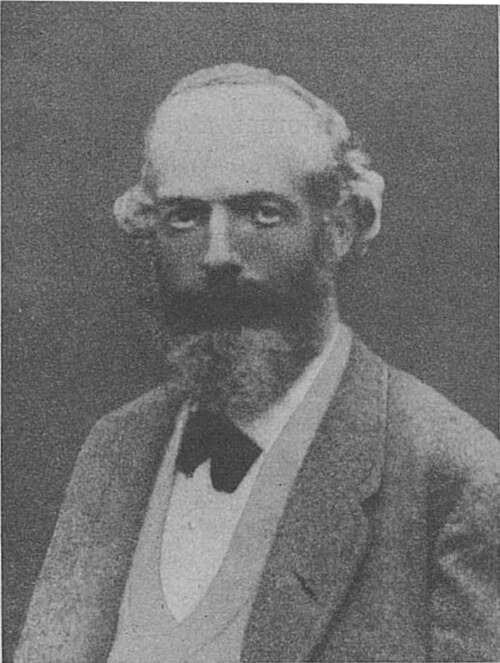
\includegraphics[width=\linewidth]{images/book3/kekule.jpg}
\end{minipage}\hfill
\begin{minipage}[t]{0.74\linewidth}
\vspace{0pt}
Em 1865, August Kekulé propôs que os seis átomos de carbono do benzeno formam
um anel com ligações simples e duplas alternadas e, pouco depois, que as duas
alternâncias se trocam tão depressa que todas as ligações são iguais. As
ligações iguais encontradas por difração de raios X e os orbitais $\pi$
estendidos sobre o anel inteiro deram à sua intuição a forma moderna; a \omterm{thm:b2:huckel:huckel-rule}{regra
de Hückel}, em 1931, explicou por que seis elétrons, e não quatro ou oito,
tornam um anel especial. (Retrato, 1873, autor desconhecido, domínio público,
Wikimedia Commons.)
\end{minipage}
\end{history}

\section{Conjugação e luz}

\begin{proposition}[A diferença de energia de um polieno]\label{prop:b2:huckel:gap}
Em um polieno linear de $n$ carbonos ($n$ par), a diferença entre o nível $\pi$
ocupado mais alto e o vazio mais baixo é $4|\beta|\sin(\pi/(2(n + 1)))$: ela
diminui à medida que a cadeia se alonga.
\end{proposition}

\begin{proof}
O nível ocupado mais alto é $k = n/2$; o vazio mais baixo, $k = n/2 + 1$. Com $\theta_k =
k\pi/(n + 1)$, $E_{n/2+1} - E_{n/2} = 2|\beta|(\cos\theta_{n/2} - \cos\theta_{n/2+1}) = 4|\beta|
\sin\frac{\theta_{n/2} + \theta_{n/2+1}}{2}\sin\frac{\theta_{n/2+1} - \theta_{n/2}}{2}$, e o
primeiro seno vale $\sin(\pi/2) = 1$. Ela diminui com $n$, pois $\sin$ é crescente em
$[0, \pi/2]$.
\end{proof}

\begin{omfigure}
\begin{tikzpicture}
\begin{axis}[width=0.5\linewidth, height=5cm, xmin=0, xmax=22, ymin=0, ymax=2.2,
  axis x line=bottom, axis y line=left, xlabel={carbonos $n$}, ylabel={diferença$/|\beta|$},
  tick label style={font=\small}, label style={font=\small}]
\addplot[omThm, thick, mark=*, mark size=1.3pt] table[x=n, y=gap] {figdata/out/bachelor-2-huckel-b.dat};
\end{axis}
\end{tikzpicture}\hfill
\begin{tikzpicture}
\begin{axis}[width=0.48\linewidth, height=5.4cm, xmin=-1, xmax=11, ymin=-2.4, ymax=2.4,
  axis x line=none, axis y line=left, ylabel={$(E - \alpha)/|\beta|$}, clip=false,
  tick label style={font=\small}, label style={font=\small}]
\addplot[only marks, mark=-, mark size=5pt, very thick, omDef] table[x=x, y=e] {figdata/out/bachelor-2-huckel-a.dat};
\draw[densely dotted] (axis cs:-1,0) -- (axis cs:11,0);
\node[anchor=north, font=\scriptsize] at (axis cs:0,-2.45) {C$_2$};
\node[anchor=north, font=\scriptsize] at (axis cs:2,-2.45) {C$_3$};
\node[anchor=north, font=\scriptsize] at (axis cs:4,-2.45) {C$_4$};
\node[anchor=north, font=\scriptsize] at (axis cs:6,-2.45) {C$_6$};
\node[anchor=north, font=\scriptsize] at (axis cs:8,-2.45) {anel 4};
\node[anchor=north, font=\scriptsize] at (axis cs:10,-2.45) {anel 6};
\end{axis}
\end{tikzpicture}

{\small À esquerda: a diferença de Hückel dos polienos lineares cai à medida
que a cadeia cresce, a razão pela qual as longas cadeias conjugadas absorvem
em comprimentos de onda maiores, até o visível. À direita: níveis calculados do
eteno, do alila, do butadieno, do hexatrieno (cadeias) e do ciclobutadieno e
do benzeno (anéis); níveis ligantes abaixo de $\alpha$.}
\end{omfigure}

Um heteroátomo é introduzido mudando sua \omterm{def:b2:diatomic-mos:integrals}{integral de Coulomb}, $\alpha_X = \alpha + h\beta$, e
as \omterm{def:b2:diatomic-mos:integrals}{integrais de ressonância} de suas ligações: um modelo com parâmetros
ajustáveis, que conserva os resultados qualitativos (um átomo eletronegativo,
$h > 0$, atrai para si a densidade $\pi$), mas cujos números são ajustados, e
não deduzidos.

\section{Exercícios}

\begin{exercise}[$\star$]\label{exo:b2:huckel:1}
Dê $E_\pi$ do cátion, do radical e do ânion alila.
\end{exercise}

\begin{exercise}[$\star$]\label{exo:b2:huckel:2}
Calcule $E_\pi$ do butadieno a partir dos níveis $\alpha \pm 1.618\beta$, $\alpha \pm 0.618\beta$.
\end{exercise}

\begin{exercise}[$\star$]\label{exo:b2:huckel:3}
\omterm{def:b2:huckel:aromatic}{Aromático}, \omterm{def:b2:huckel:aromatic}{antiaromático} ou nenhum dos dois (se plano): benzeno, ânion
ciclopentadienila, cátion ciclopentadienila, cátion tropílio \ce{C7H7+},
ciclobutadieno, ciclo-octatetraeno plano.
\end{exercise}

\begin{exercise}[$\star$]\label{exo:b2:huckel:4}
Desenhe o círculo de Frost do ciclo-octatetraeno plano e coloque seus oito elétrons $\pi$.
\end{exercise}

\begin{exercise}[$\star\star$]\label{exo:b2:huckel:5}
Calcule a \omterm{def:b2:huckel:delocalisation}{energia de deslocalização} do butadieno e dê-a em \unit{kJ/mol} com
$|\beta| = \qty{75}{kJ/mol}$. Compare com os \qty{10}{kJ/mol} dos dados de
hidrogenação do ciclo-hexa-1,3-dieno.
\end{exercise}

\begin{exercise}[$\star\star$]\label{exo:b2:huckel:6}
Calcule os índices de ligação $\pi$ do butadieno e preveja qual de suas
ligações C--C é a mais curta.
\end{exercise}

\begin{exercise}[$\star\star$]\label{exo:b2:huckel:7}
Os níveis de um anel de cinco membros são $\alpha + 2\beta$, $\alpha + 0.618\beta$ (duas vezes),
$\alpha - 1.618\beta$ (duas vezes). Preencha-os para o ânion e o cátion
ciclopentadienila e compare.
\end{exercise}

\begin{exercise}[$\star\star$]\label{exo:b2:huckel:8}
Usando os níveis de um anel de sete membros, explique por que o brometo de
ciclo-heptatrienila se comporta como um sal, o brometo de tropílio.
\end{exercise}

\begin{exercise}[$\star\star$]\label{exo:b2:huckel:9}
Verifique a regra do traço no hexatrieno, cujos níveis são $\alpha \pm 1.802\beta$, $\alpha \pm
1.247\beta$, $\alpha \pm 0.445\beta$.
\end{exercise}

\begin{exercise}[$\star\star\star$]\label{exo:b2:huckel:10}
Deduza os níveis do hexatrieno a partir da fórmula fechada, e sua \omterm{def:b2:huckel:delocalisation}{energia de deslocalização}.
\end{exercise}

\begin{exercise}[$\star\star\star$]\label{exo:b2:huckel:11}
O ciclobutadieno quadrado teria dois elétrons desemparelhados. Explique por que
a molécula real é retangular, com duas ligações curtas e duas longas.
\end{exercise}

\begin{exercise}[$\star\star\star$]\label{exo:b2:huckel:12}
Em um sistema $\pi$ de dois átomos \ce{C=X} com $\alpha_X = \alpha + \beta$ (valor de modelo, $h = 1$) e
$\beta_{\ce{CX}} = \beta$, encontre os dois níveis e as cargas $\pi$ em C e em X para
dois elétrons.
\end{exercise}

\section{Problema: A energia que falta ao benzeno}

\begin{problem}[{Problema de fim de semana --- a estabilização aromática do benzeno a
partir das entalpias de hidrogenação, os níveis de Hückel do benzeno e sua
energia de deslocalização, o valor de $|\beta|$, e a comparação com o hexatrieno
e o ciclo-octatetraeno}]
\label{pb:b2:huckel:1}
Dados: entalpias de formação dos gases (\unit{kJ/mol}): benzeno 82.9,
ciclo-hexa-1,3-dieno 104.6, ciclo-hexeno $-4.3$, ciclo-hexano $-123.1$.
Comprimentos de ligação (pm): benzeno 139.7, eteno 133.9, etano 153.6.
% ledger: dfh:C6H6_g, dfh:C6H8_g, dfh:C6H10_g, dfh:C6H12_g, geo:C6H6.rCC, geo:C2H4.rCC, geo:C2H6.rCC

\medskip
\noindent\textbf{Parte I --- A hidrogenação.}
\begin{enumerate}
  \item Calcule o $\Delta_r H^\circ$ da hidrogenação do ciclo-hexeno a ciclo-hexano.
  \item O mesmo para o ciclo-hexa-1,3-dieno.
  \item O mesmo para o benzeno.
  \item O que três ligações duplas independentes liberariam?
  \item Deduza a estabilização do benzeno.
  \item Compare com a do dieno conjugado e comente.
\end{enumerate}

\medskip
\noindent\textbf{Parte II --- O benzeno de Hückel.}
\begin{enumerate}[resume]
  \item Escreva a matriz de Hückel do benzeno.
  \item Dê seus níveis pela fórmula do anel.
  \item Preencha-os com seis elétrons $\pi$.
  \item Calcule $E_\pi$.
  \item Calcule o $E_\pi$ de três ligações duplas isoladas.
  \item Deduza a \omterm{def:b2:huckel:delocalisation}{energia de deslocalização}.
  \item Verifique a regra do traço.
\end{enumerate}

\medskip
\noindent\textbf{Parte III --- O valor de $|\beta|$.}
\begin{enumerate}[resume]
  \item Iguale a \omterm{def:b2:huckel:delocalisation}{energia de deslocalização} à estabilização da Parte I e encontre
        $|\beta|$.
  \item Com esse valor, preveja a \omterm{def:b2:huckel:delocalisation}{energia de deslocalização} do butadieno e
        compare com a Parte I.
  \item Calcule os índices de ligação $\pi$ do benzeno.
  \item Compare-os com os do butadieno.
  \item Explique por que os comprimentos de ligação do benzeno são iguais e
        onde eles se situam.
\end{enumerate}

\medskip
\noindent\textbf{Parte IV --- Outros anéis e cadeias.}
\begin{enumerate}[resume]
  \item Calcule a \omterm{def:b2:huckel:delocalisation}{energia de deslocalização} do hexatrieno e compare com o benzeno.
  \item Dê os níveis do ciclo-octatetraeno plano.
  \item Preencha-os com oito elétrons: o que há de errado?
  \item Como a molécula real escapa?
  \item Qual é a situação do ciclobutadieno?
  \item Enuncie a \omterm{thm:b2:huckel:huckel-rule}{regra de Hückel}.
  \item Dê o valor de $|\beta|$ obtido igualando a \omterm{def:b2:huckel:delocalisation}{energia de deslocalização} do
        benzeno à sua estabilização medida.
\end{enumerate}
\end{problem}
